\documentclass[../notes.tex]{subfiles}

\pagestyle{main}
\renewcommand{\chaptermark}[1]{\markboth{\chaptername\ \thechapter\ (#1)}{}}

\begin{document}




\chapter{Pyridine Chemistry}
\section{Intro, Directed Metallation, and Organometallic Coupling}
\begin{itemize}
    \item \marginnote{1/4:}Announcements.
    \begin{itemize}
        \item This class is a survey course; it is not comprehensive.
        \item This class has a different philosophy from mainstream heterocyclic chemistry; we'll focus not on the "coolest" chemistry, but the chemistry that actually gets used.
        \begin{itemize}
            \item Focus on \emph{Journal of Medicinal Chemistry} and process chem journals.
            \item Steve does not believe that academic research has to be useful, but\dots
            \item Steve believes: Proof is in the pudding. If you're pretending what you're doing has some practical application, you should see it going after 5 years.
        \end{itemize}
        \item Grader: Dr. Dennis Kutateladze.
        \begin{itemize}
            \item He grades the 2 exams; Steve writes both of them.
        \end{itemize}
        \item There are PSets (ungraded, but keys posted).
        \item This is supposed to be a very low-key class; getting a good grade should be easy.
        \begin{itemize}
            \item The goal is to expose you to a lot of different useful chemistry.
            \item Don't look up PSets; goal is not to impress Steve, but to learn the material.
        \end{itemize}
        \item 2 exams + project; (project is graded for completion and effort).
        \begin{itemize}
            \item With 20+ students, probably all of the last 3 classes will be dedicated to presentations.
        \end{itemize}
        \item \textcite{bib:JouleMills} is somewhat dated.
        \begin{itemize}
            \item "A lot of heterocyclic chemistry is ancient."
        \end{itemize}
        \item Organometallic methods come a bit more to the fore in this rendition because Allison isn't currently teaching 5.44 - Organometallic Chemistry.
        \item The final project.
        \begin{itemize}
            \item Most drugs come from the new FDA approvals from last year.
            \item We should put together a 10-minute PowerPoint presentation in which we discuss the disease, how it was discovered, the MedChem synthesis, the process synthesis, the competitors, etc. Emphasis on medchem and process syntheses.
            \item Look at patents, primary papers, etc. Do \emph{not} find a review article and summarize it.
            \item Goal: If we were interested in a compound for our research or job, how would we go about finding material on it?
        \end{itemize}
    \end{itemize}
    \item Mostly looking at aromatic heterocycles, e.g., not piperidines or tetrahydrofurans.
    \begin{figure}[H]
        \centering
        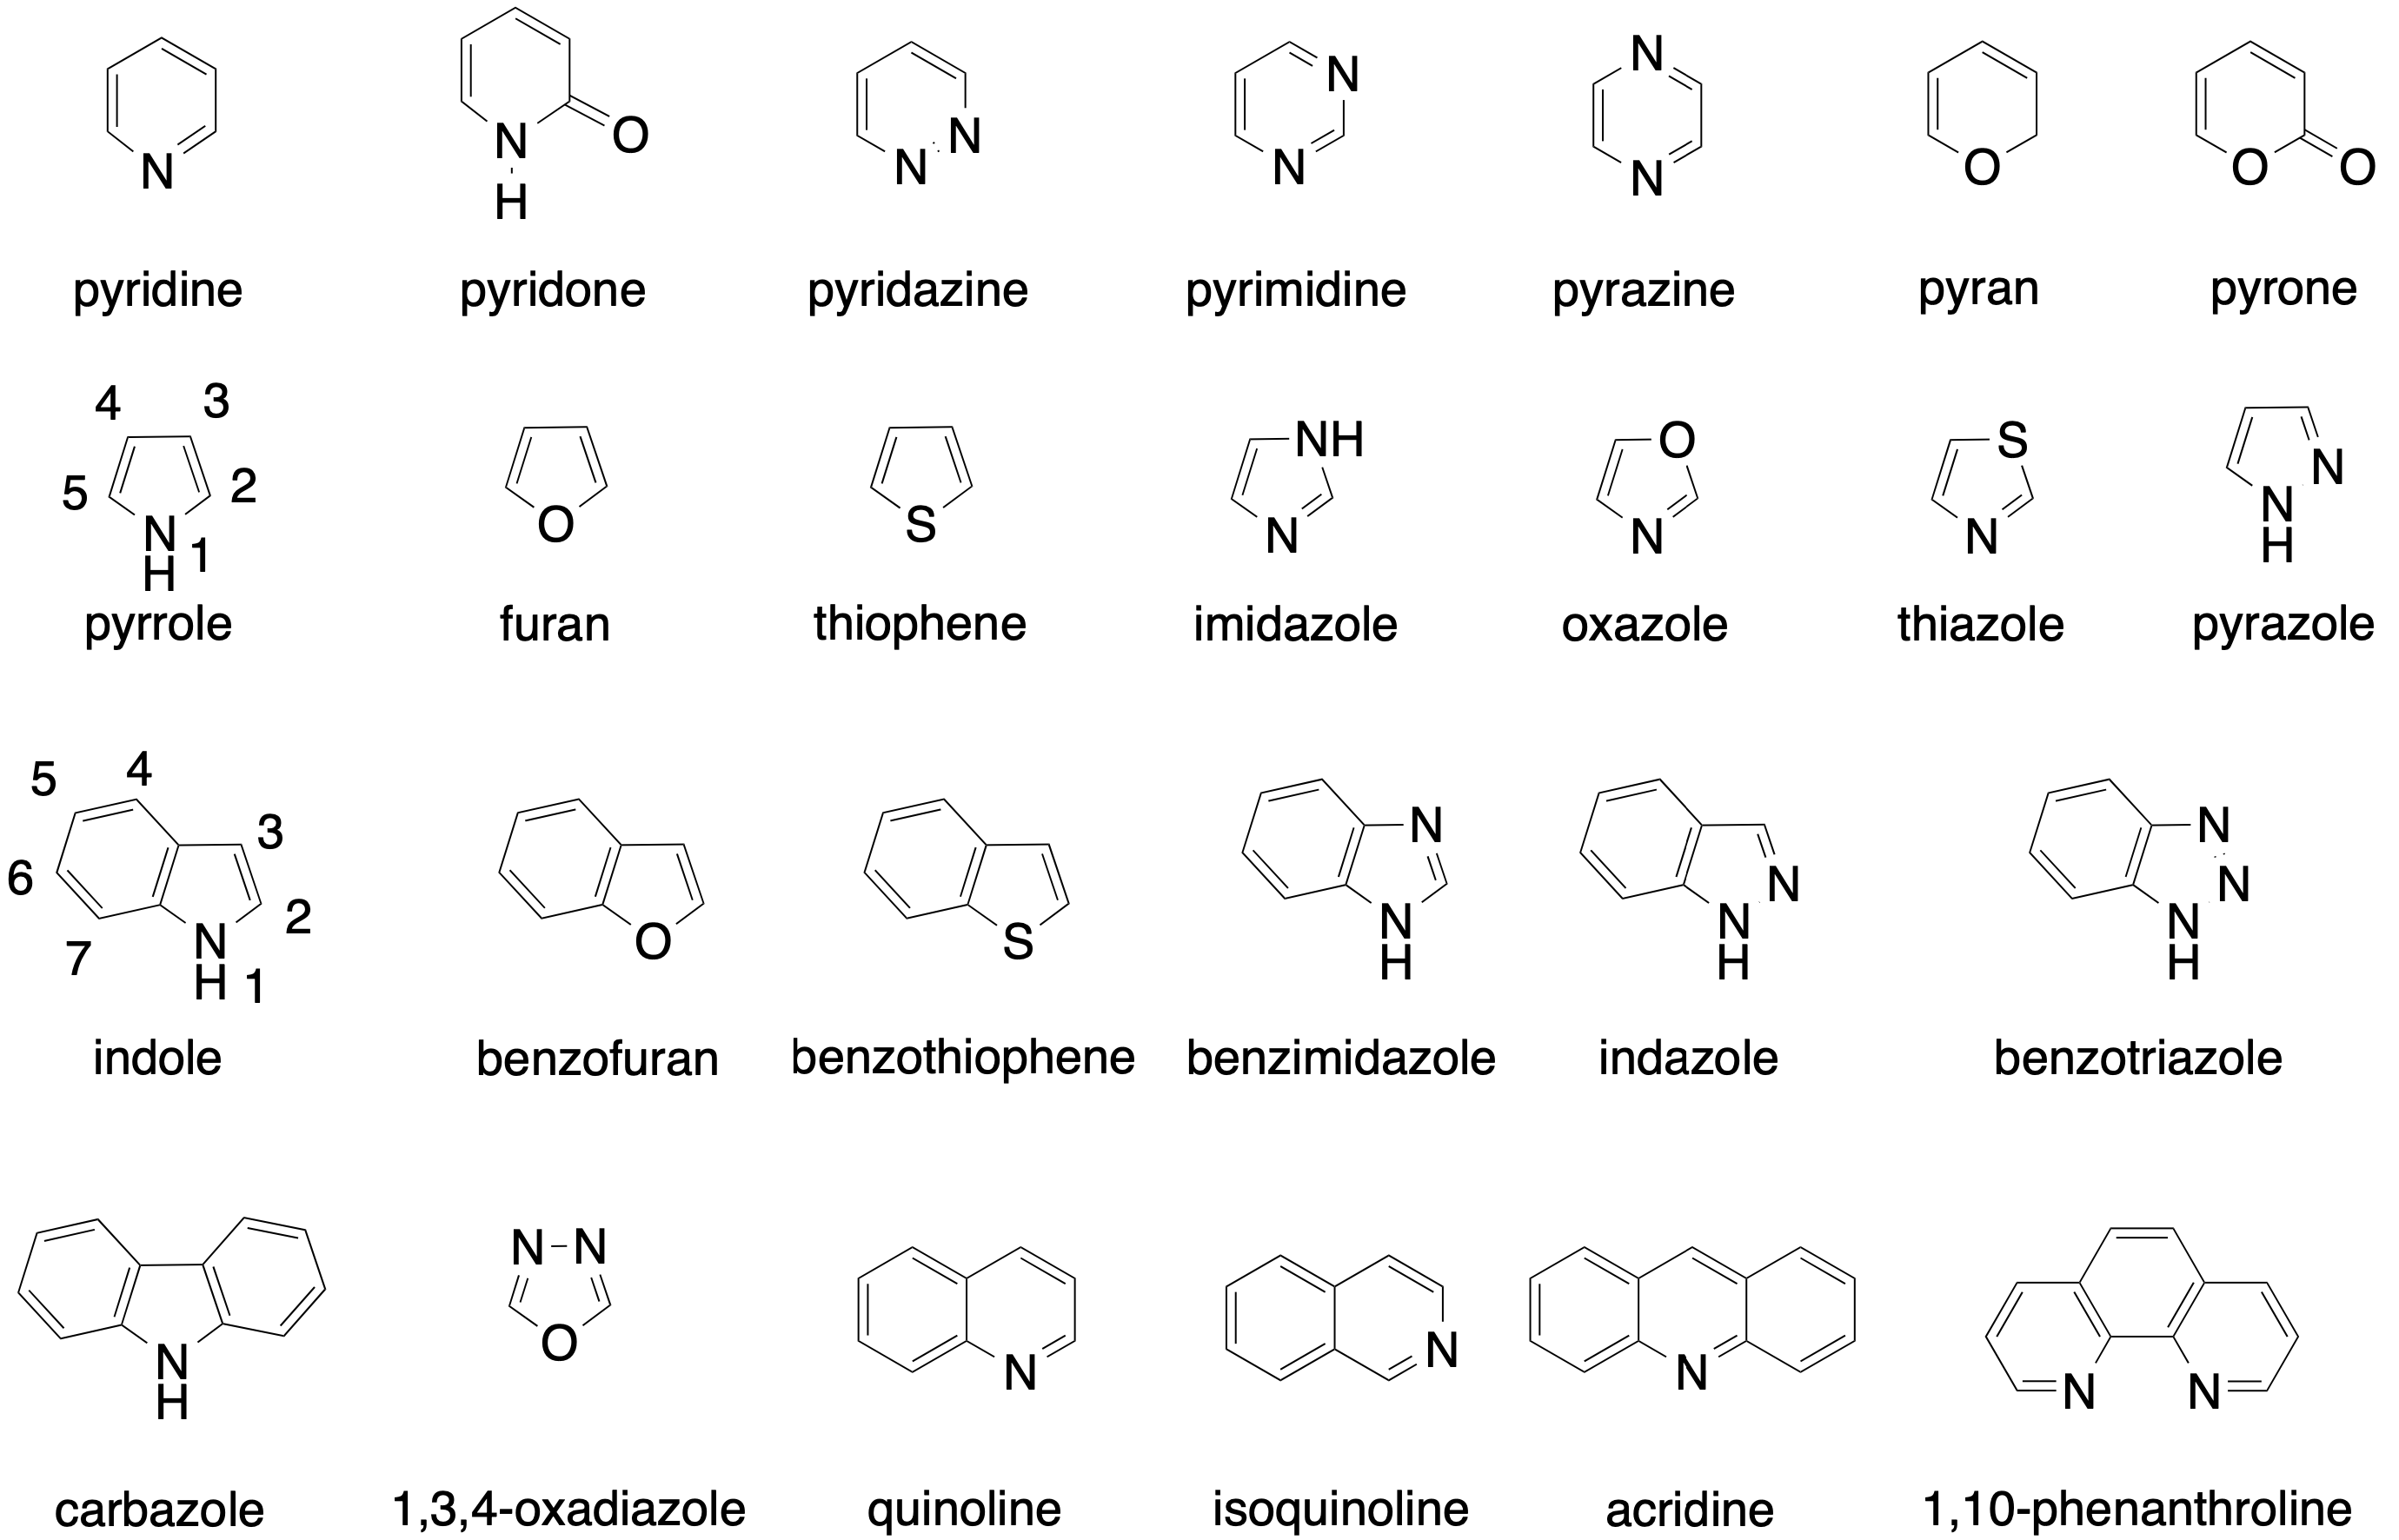
\includegraphics[width=0.8\linewidth]{heterocycles.png}
        \caption{Heterocycles of interest.}
        \label{fig:heterocycles}
    \end{figure}
    \begin{itemize}
        \item We don't need to know the names of all the heterocycles, but we should learn the big ones!!
        \item Interesting heterocycles often contain because it can be protonated, and it hydrogen bonds.
        \begin{itemize}
            \item Hydrogen bonding is useful for receptors, salt bridges, etc.
        \end{itemize}
        \item Salts of these compounds usually imply some kind of water solubility.
        \item \textbf{Pharmacokinetics} are often moderated by heterocycles.
        \begin{itemize}
            \item Making the drug hang around for the right amount of time is super important, because the more times per day people have to take the drugs, the more that compliance goes down (especially among the elderly population).
        \end{itemize}
    \end{itemize}
    \item Blockbuster drugs.
    \begin{itemize}
        \item Several examples given.
        \item Imbruvica Janssen is a covalent drug, doing a Michael addition to DNA.
    \end{itemize}
    \item Infamous drugs.
    \begin{itemize}
        \item Lipitor.
        \begin{itemize}
            \item A \textbf{statin}, i.e., a cholesterol-lowering agent.
            \item One of the most important drugs in the last century in extending people's lifetimes.
            \item Anyone over 50 either has taken one (or should take one, in Steve's opinion!).
        \end{itemize}
        \item Quinine.
        \begin{itemize}
            \item Anti-malarial.
            \item Also in gin and tonics!
        \end{itemize}
        \item Strychnine.
        \begin{itemize}
            \item Rat poison.
            \item Big target in synthetic chemistry, starting with Woodward.
        \end{itemize}
        \item $\beta$-lactam antibiotics.
        \begin{itemize}
            \item Penicillin, and the ring-expanded cephalexins.
        \end{itemize}
        \item Thalidomide.
        \begin{itemize}
            \item Caused the big push for the sale of single-enantiomer drugs!
        \end{itemize}
    \end{itemize}
    \item Pyridine.
    \begin{itemize}
        \item Horrible-smelling, polar solvent.
        \item Originally came from coal tar (precursor to petroleum).
    \end{itemize}
    \item Current synthesis of pyridine.
    \begin{equation*}
        \ce{CH3CHO + H2CO + NH3 ->[vapor phase][Si/Al cat] Py + 3-MePy}
    \end{equation*}
    \begin{itemize}
        \item This synthesis is carried out with flow chemistry.
        \begin{itemize}
            \item Before it was trendy in pharma, it is the only thing that was \emph{ever} used in the production of commodity chemicals.
            \item When you're making commodity chemicals, you can't afford solvents or separations.
        \end{itemize}
        \item It produces pyridine on a scale of 20,000 tons per year.
    \end{itemize}
    \item Aside: Many chemicals are produced from such "magic reactions."
    \begin{itemize}
        \item Example: Acrylonitrile.
        \begin{itemize}
            \item Industrial synthesis: Mix propene and ammonia with a molybdenum/vanadium catalyst.
        \end{itemize}
        \item Example: THF.
        \begin{itemize}
            \item Industrial synthesis: From butane!
        \end{itemize}
        \item "I mean, how?! Write a mechanism for that!"
    \end{itemize}
    \item Many drugs contain pyridine moieties. Here are some examples.
    \begin{itemize}
        \item Muscopyridine: Perfumes.
        \item Prevacid: Acid reflux.
        \item Nexium: Sold as a single-enantiomer with a stereogenic sulfur atom!
    \end{itemize}
    \item The pharmaceutical industry is largely focused on old people because it's a huge market share.
    \begin{itemize}
        \item Pain, sleep, etc. are huge.
        \item As you get older, your body starts to break down.
        \item Alzheimers is a big target, but not much success so far.
    \end{itemize}
    \item The structure of pyridine.
    \begin{figure}[H]
        \centering
        \begin{subfigure}[b]{\linewidth}
            \centering
            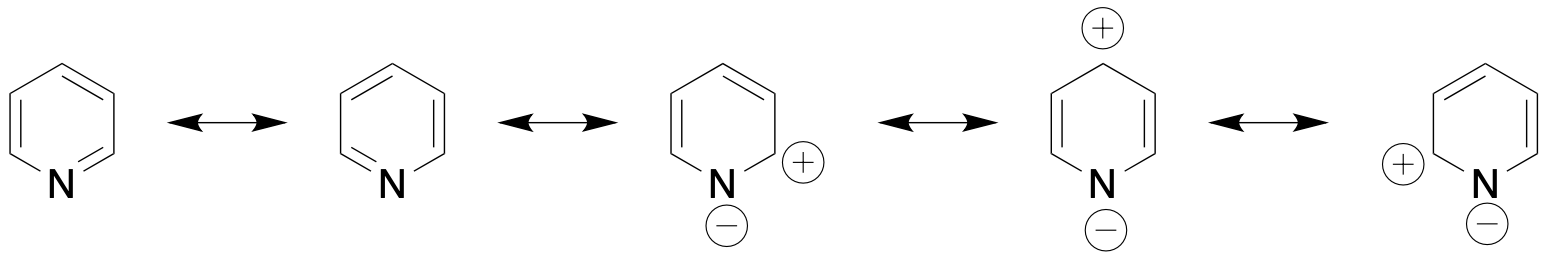
\includegraphics[width=0.7\linewidth]{PyStructurea.png}
            \caption{Important resonance forms.}
            \label{fig:PyStructurea}
        \end{subfigure}\\[1em]
        \begin{subfigure}[b]{0.3\linewidth}
            \centering
            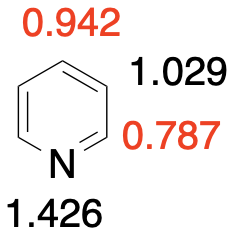
\includegraphics[width=0.39\linewidth]{PyStructureb.png}
            \caption{$\pi$-electron populations.}
            \label{fig:PyStructureb}
        \end{subfigure}
        \begin{subfigure}[b]{0.3\linewidth}
            \centering
            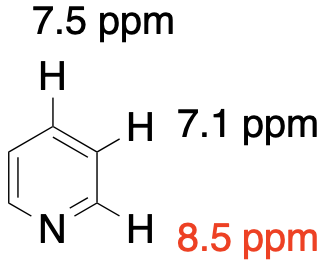
\includegraphics[width=0.55\linewidth]{PyStructurec.png}
            \caption{\ce{{}^1H} NMR shifts.}
            \label{fig:PyStructurec}
        \end{subfigure}
        \caption{Pyridine structure.}
        \label{fig:PyStructure}
    \end{figure}
    \begin{itemize}
        \item Analogous to benzene; slightly less aromatic, but very similar.
        \item Insights from the \ce{{}^1H} NMR.
        \begin{itemize}
            \item \emph{ortho}-proton shifts significantly downfield, \emph{meta}-proton is largely unaffected, and \emph{para}-proton shifts downfield a bit.
            \item This is because there are resonance structures where we put $\delta^+$ on the 2,4,6-positions, while the \emph{meta}-positions take a slight $\delta^-$.
        \end{itemize}
        \item Strong dipole (\SI{2.2}{\debye}) toward the nitrogen atom.
        \item More $\pi$-electron density on nitrogen than anything else.
    \end{itemize}
    \item Reactivity of pyridine.
    \begin{itemize}
        \item Can be reduced to piperidines, sometimes with selectivity, sometimes enantioselectively.
        \item Minisci-type radical reactions.
        \item As an electrophile.
        \item As a Lewis base.
        \item As a Br\o nsted base.
        \item As a nucleophile.
        \item As a reductant.
        \item Very different electrophilic aromatic substitution (EAS) reactivity compared to benzene. You really need activating EDGs with pyridine!
        \item Nucleophilicity is most likely to happen at the nitrogen atom.
        \item S\textsubscript{N}Ar is most likely to happen at the electron-deficient 2,4,6-positions.
        \item EAS is most likely to happen at the relatively electron-rich \emph{meta}-positions.
    \end{itemize}
    \item Pyridine as a base or nucleophile.
    \begin{itemize}
        \item $\pKa\approx 5.5$; much less basic than piperidine.
        \item Basicicity is modulated by EDGs/EWGs.
        \item Pyridine can be transformed from a good to a great nucleophile with some EDGs, e.g., with DMAP.
        \begin{itemize}
            \item DMAP provides rate enhancements of up to $10^4$.
        \end{itemize}
    \end{itemize}
    \item Pyridine reactivity trends.
    \begin{itemize}
        \item Much of pyridine reactivity is driven by\dots
        \begin{itemize}
            \item Avoiding a $\delta^+$ charge on \ce{N}.
            \item That pyridine is a $\pi$-deficient heterocycle (like pyrrole).
        \end{itemize}
        \item Brute force conditions can yield sulfonation.
        \begin{itemize}
            \item The nitrogen would usually react with the electrophile first, and then the product is $10^8$ times less reactive than pyridine, alone.
        \end{itemize}
    \end{itemize}
    \item Nucleophilic aromatic substitution (S\textsubscript{N}Ar) with pyridine.
    \begin{itemize}
        \item Much better with pyridine than with benzene!
        \item Charged intermediates (e.g., where the \ce{N} has coordinated to \ce{E+}) react \emph{exceptionally} fast.
        \item 2,4-chloro is better because you can delocalize the negative charge onto the nitrogen.
    \end{itemize}
    \item Example pyridine reactivity: Biological oxidation of alcohols to aldehydes.
    \begin{itemize}
        \item Done with \ce{NAD+} and a pyridine derivative!
    \end{itemize}
    \item Pyridones.
    \begin{figure}[H]
        \centering
        \footnotesize
        \schemestart
            \chemfig{*6(-N=(-OH)-=-=)}
            \arrow{<->>}
            \chemfig{*6(-\chembelow{N}{H}-(=O)-=-=)}
        \schemestop
        \caption{Pyridone tautomerization.}
        \label{fig:pyridoneTaut}
    \end{figure}
    \begin{itemize}
        \item 2-pyridone (Figure \ref{fig:pyridoneTaut}): Both tautomers are aromatic, but pyridone has stronger BDEs.
        \item 4-pyridone: Still the ketone form.
        \item 3-pyridone: Forms the zwitterion.
    \end{itemize}
    \item Pyridone reactivity.
    \begin{figure}[h!]
        \centering
        \footnotesize
        \begin{subfigure}[b]{\linewidth}
            \centering
            \schemestart
                \chemfig{*6(-\chembelow{N}{H}(-[6,0.4,,,opacity=0])-(=O)-=-=)}
                \arrow{->[\ce{POCl3}][base]}[,1.2]
                \chemfig{*6(-N(-[6,0.4,,,opacity=0])=(-Cl)-=-=)}
            \schemestop
            \caption{The reaction.}
            \label{fig:pyridoneCla}
        \end{subfigure}\\[2em]
        \begin{subfigure}[b]{\linewidth}
            \centering
            \schemestart
                \chemfig{*6(-N(-[@{11}]@{1H}H)-[@{12,0.4}](=[@{13}]O)-=-=)}
                \arrow{->[{\chemfig[atom sep=1.4em]{@{2P}P(=[2]O)(-[@{21}:-30]@{2Cl}Cl)(-[6]Cl)(-[:-150]Cl)}}][\chemfig{@{3B}\charge{180=\:}{B}}]}[,1.6]
                \chemfig{*6(-@{4N}N(-[,,,,opacity=0]\phantom{H})=[@{41}]@{4C}(-O-[:30]POCl_2)-(-[:20,0.5,,,opacity=0]@{4Cl}\charge{[extra sep=4pt]45=$\ominus$}{Cl})=-=)}
                \arrow
                \chemfig{*6(-@{5N}\charge{[extra sep=5pt]-90=$\ominus$}{N}(-[,,,,opacity=0]\phantom{H})-[@{51}](-[@{52}:-50]O-[@{53}:10]POCl_2)(-[:-10]Cl)-=-=)}
                \arrow{->[-\ce{PO2Cl}][-\ce{HCl}]}[,1.3]
                \chemfig{*6(-N(-[6,0.4,,,opacity=0])=(-Cl)-=-=)}
            \schemestop
            \chemmove{
                \draw [curved arrow={6pt}{2pt}] (3B) to[out=180,in=0] (1H);
                \draw [curved arrow={2pt}{2pt}] (11) to[bend right=60,looseness=1.5] (12);
                \draw [curved arrow={3pt}{2pt}] (13) to[out=60,in=150] (2P);
                \draw [curved arrow={2pt}{2pt}] (21) to[bend left=80,looseness=3] (2Cl);
                % 
                \draw [curved arrow={10pt}{2pt}] (4Cl) to[out=45,in=25,out looseness=2,in looseness=4] (4C);
                \draw [curved arrow={4pt}{2pt}] (41) to[bend right=80,looseness=3] (4N);
                % 
                \draw [curved arrow={10pt}{2pt}] (5N) to[out=-90,in=-70,out looseness=4.5,in looseness=4] (51);
                \draw [curved arrow={2pt}{2pt}] (52) to[bend right=100,looseness=2.5] (53);
            }
            \caption{The mechanism.}
            \label{fig:pyridoneClb}
        \end{subfigure}
        \caption{Pyridone chlorination.}
        \label{fig:pyridoneCl}
    \end{figure}
    \begin{itemize}
        \item \ce{POCl3} is one of the most used species in heterocyclic chemistry.
        \item It works so well because \ce{P=O} bond formation is an \emph{excellent} driving force.
    \end{itemize}
    \item Directed metallation --- see \textcite{bib:5-511Notes}.
    \begin{itemize}
        \item Has been around for a while.
        \begin{itemize}
            \item Sigma-Aldrich catalogs have thousands of monosubstituted aromatics, probably still thousands of disubstituted aromatics, but very few (very expensive) tri-substituted aromatics.
            \item Example: Buy anisole, and then you can very easily upgrade it with directed metallation.
        \end{itemize}
        \item Pioneers: Victor Snieckus (Queen's University) and Peter Beak (UIUC).
        \item Two mechanistic theories: Binding to the functional group, and an inductive effect of acidification.
        \begin{itemize}
            \item An expert in lithium chemistry at Cornell has shown that the inductive effect is more important, at least in the case of anisole, contrary to 5.511!
        \end{itemize}
        \item Per Steve, this is one of the most important transformations in organic chemistry.
        \item Common directing groups.
        \begin{itemize}
            \item Aryl ethers, $3^\circ$ amides, MOM ethers, $3^\circ$ carbamates, and $3^\circ$ sulfonamides.
            \item For $\pi$-deficient heterocycles (e.g., pyridine), also: \ce{F}, \ce{Cl}, \ce{Br}, \ce{CF3}, \ce{CO2-}.
        \end{itemize}
        \item References: \textcite{bib:DMGRev1}, \textcite{bib:DMGRev2}, \textcite{bib:DMGRev3}.
    \end{itemize}
    \pagebreak
    \item Pyridine preferably undergoes metallation \emph{not} adjacent to the nitrogen.
    \begin{itemize}
        \item \ce{N-Li} binding kinetically favors lithiation at the \emph{ortho}-positions.
        \item However, having two lone pairs so close together is thermodynamically disfavored, presumably because of Coulombic repulsion between the electron pairs, i.e., the \textbf{$\bm{\alpha}$-effect}.
        \item Indeed, lithiation actually prefers to happen at the more acidic \emph{para}-position, which is still $\delta^+$ but has less coulombic repulsion.
        \item Remember that $\pKa$ is a \emph{thermodynamic} function.
    \end{itemize}
    \item DMGs on pyridine.
    \begin{itemize}
        \item Most \emph{meta}-DMGs direct to the \emph{para}-position: \ce{Cl}, \ce{F}, MOM ethers, siloxane ethers, bulky $3^\circ$ amides (e.g., \ce{C(O)N{}^{\emph{i}}Pr2}), and bulky amides bonded through the nitrogen.
        \item \emph{meta}-\ce{OEt} directs to the \emph{ortho}-position.
        \item Review some typical lithiation and functionalization reactions from 5.511.
        \begin{itemize}
            \item LDA lithiates 3-chloropyridine at $-\SI{23}{\celsius}$ instead of eliminating to the benzyne derivative (as it would at a higher temperature).
        \end{itemize}
        \item References lithium halogen exchange.
    \end{itemize}
    \item Lateral deprotonations.
    \begin{itemize}
        \item \emph{ortho}- and \emph{para}-methylpyridine like to deprotonate "benzylically" much more than toluene because of additional nitrogen stabilization.
        \begin{itemize}
            \item Indeed, the $\pKa$ of the 2,3,4-positions is 29.5, 33.5, and 26, respectively.
            \item In contrast, toluene's $\pKa$ is 42.
        \end{itemize}
        \item Decarboxylation can be useful for substitution reactions.
        \begin{itemize}
            \item Example: Mixing 2-pyridylacetic acid with a base leads to decarboxylation and the formation of 2-methylpyridine upon workup.
        \end{itemize}
        \item Thermodynamic vs. kinetic lateral deprotonations.
        \begin{itemize}
            \item Consider 2,4-dimethylpyridine.
            \item Bases of comparable strength (e.g., LDA) deprotonate thermodynamically at the 4-position.
            \item Stronger bases with aggregates broken up by the directing nitrogen (e.g., \ce{{}^{\emph{n}}BuLi}) deprotonate kinetically at the 2-position.
            \item Interestingly, adding \ce{{}^{\emph{n}}BuLi} and then an amine base allows for equilibration from the kinetic 2-lithiated to the thermodynamic 4-lithiated species!
            \item Reference: \textcite[90]{bib:PyLatThermKin}.
        \end{itemize}
    \end{itemize}
    \item How could we convert 2-chloro to 2-methylpyridine?
    \begin{figure}[h!]
        \centering
        \vspace{-2em}
        \footnotesize
        \schemestart
            \chemfig{*6(-N=(-Cl)-=-=)}
            \arrow{0}[,0.1]\+{,,-2pt}
            \chemfig{\charge{[extra sep=5pt]180=$\ominus$}{}(-[:60]CO_2Me)(-[:-60]CO_2Me)-[4,0.5,,,opacity=0]}
            \arrow
            \chemfig{*6(-N=(-(-[:30]CO_2Me)(-[6]CO_2Me))-(-[,,,,opacity=0]-[2,,,,opacity=0]\phantom{CO_2Me})=-=)}
            \arrow{->[\ce{HO-}][$\Delta$]}
            \chemfig{*6(-N=(-Me)-=-=)}
        \schemestop
        \caption{Lateral pyridine decarboxylation in robust synthesis.}
        \label{fig:PyLatCO2}
    \end{figure}
    \begin{itemize}
        \item General rule: If you can use chemistry from the 1920s, it will work better than chemistry from the 2020s.
        \item Lab scale: Do cross-coupling with methyl boronic acid and a palladium catalyst.
        \item 100 ton scale: Use a malonate anion and then double decarboxylation.
    \end{itemize}
    \item Pyridines as ylide-like species.
    \begin{figure}[H]
        \centering
        \begin{subfigure}[b]{\linewidth}
            \centering
            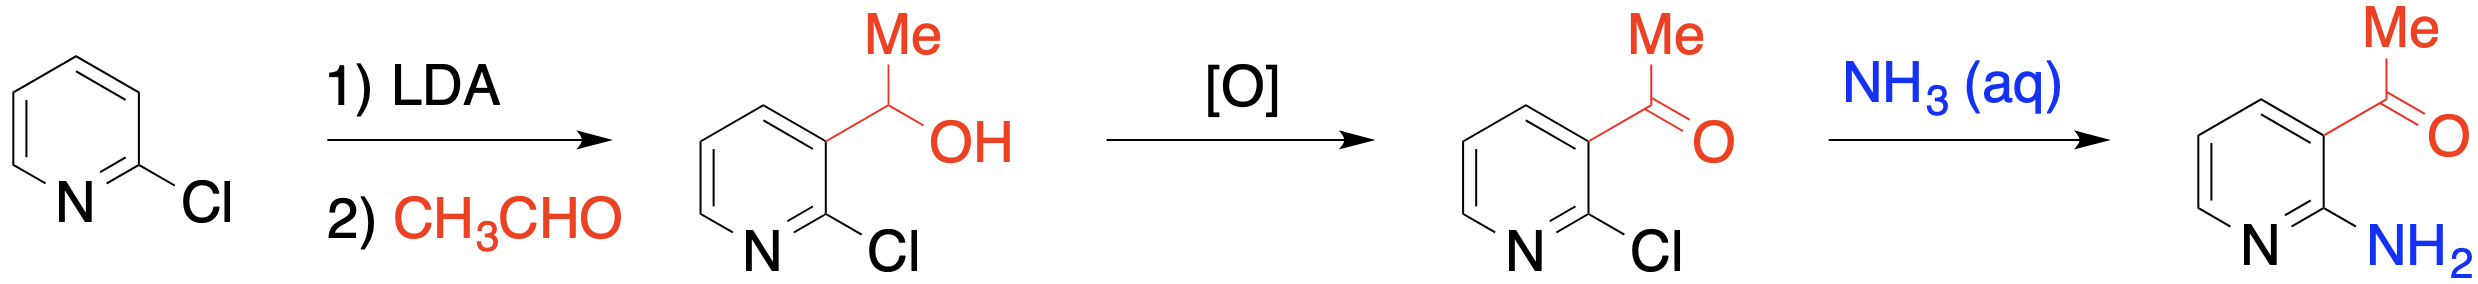
\includegraphics[width=0.85\linewidth]{PyMultifunca.png}
            \caption{Preparation of pyridyne "ylides."}
            \label{fig:PyMultifunca}
        \end{subfigure}\\[2em]
        \begin{subfigure}[b]{\linewidth}
            \centering
            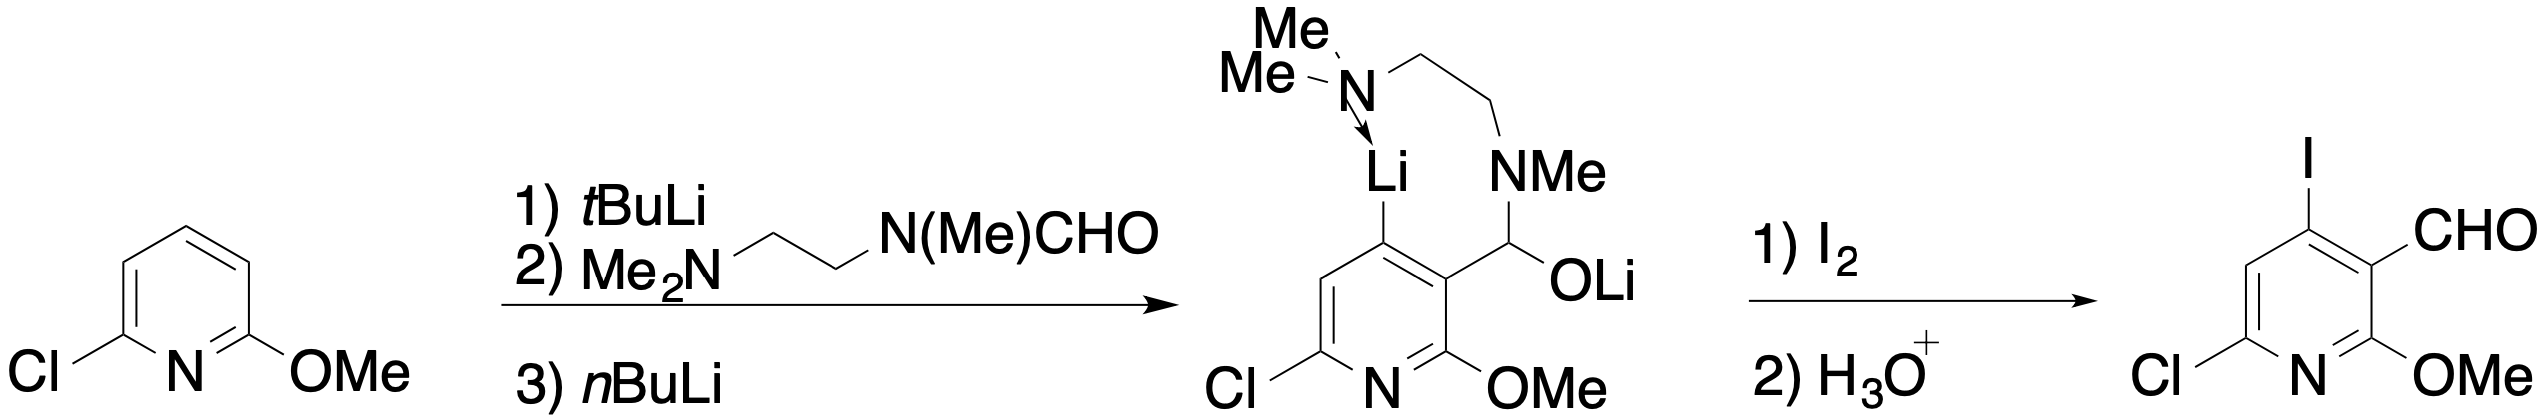
\includegraphics[width=0.85\linewidth]{PyMultifuncb.png}
            \caption{3,4-difunctionalization.}
            \label{fig:PyMultifuncb}
        \end{subfigure}
        \caption{Multifunctionalization of pyridines.}
        \label{fig:PyMultifunc}
    \end{figure}
    \begin{itemize}
        \item You can form what is essentially a ylide between the 2- and 3-positions of the pyridyne by adding an EWG adjacent to a S\textsubscript{N}Ar position (Figure \ref{fig:PyMultifunca}).
        \begin{itemize}
            \item Essentially, we begin with a species that has a DMG which can also (later on) do S\textsubscript{N}Ar.
            \item We use it as a DMG to functionalize the adjacent position with an EWG of interest.
            \item The EWG makes the ring even more activated toward S\textsubscript{N}Ar.
            \item Thus, we've essentially added a nucleophile and electrophile to pyridine very quickly.
        \end{itemize}
        \item Can get fancier with 3,4-disubstitutions (Figure \ref{fig:PyMultifuncb}).
        \begin{itemize}
            \item The stronger methoxy DMG lithiates at the 3-position. We then add a TMEDA-like species and use it to lithiate at the 4-position.
            \item An electrophile can then add at the 4-position, and we can cleave off TMEDA with an acid workup.
        \end{itemize}
        \item Steve skips the last reaction (using a \emph{para}-carbamate to asymetrically functionalize both \emph{meta}-positions).
    \end{itemize}
    \item Aside on medchem.
    \begin{itemize}
        \item \emph{Yield} and \emph{ee} are things we fixate on as academics, but medicinal chemists don't care.
        \item "People who are unsuccessful spend a lot of time optimizing something that doesn't end up working out."
        \item It's much more important to be able to get a mockup of the drug to test, and then they'll get a better working reaction later if need be.
    \end{itemize}
    \item The \textbf{Chichibabin reaction}.
    \begin{figure}[h!]
        \centering
        \footnotesize
        \schemestart
            \chemfig{*6(-N=-=-=)}
            \arrow{->[\ce{NaNH2}][\SI{160}{\celsius}, Tol]}[,1.6]
            \chemfig{*6(-N=(-NH_2)-=-=)}
        \schemestop
        \caption{Chichibabin reaction.}
        \label{fig:chichibabin}
    \end{figure}
    \begin{itemize}
        \item Makes 2-aminopyridine from pyridine.
    \end{itemize}
    \pagebreak
    \item Activating pyridine toward $sp^2$- and $sp$-Grignard reagents.
    \begin{itemize}
        \item If we treat pyridine with an acid chloride or other EWG, it adds in to form an activated `amide.'
        \item We can then easily do S\textsubscript{N}Ar at the 2-position with \ce{ArMgX}, \ce{ViMgX}, or an alkynyl Grignard.
        \item This reaction is \emph{not} selective for alkyl Grignards.
    \end{itemize}
    \item Pyridine isn't very good at EAS, but pyridine \emph{N}-oxide can do it better.
    \item Synthesis of a pyridine \emph{N}-oxide.
    \begin{figure}[h!]
        \centering
        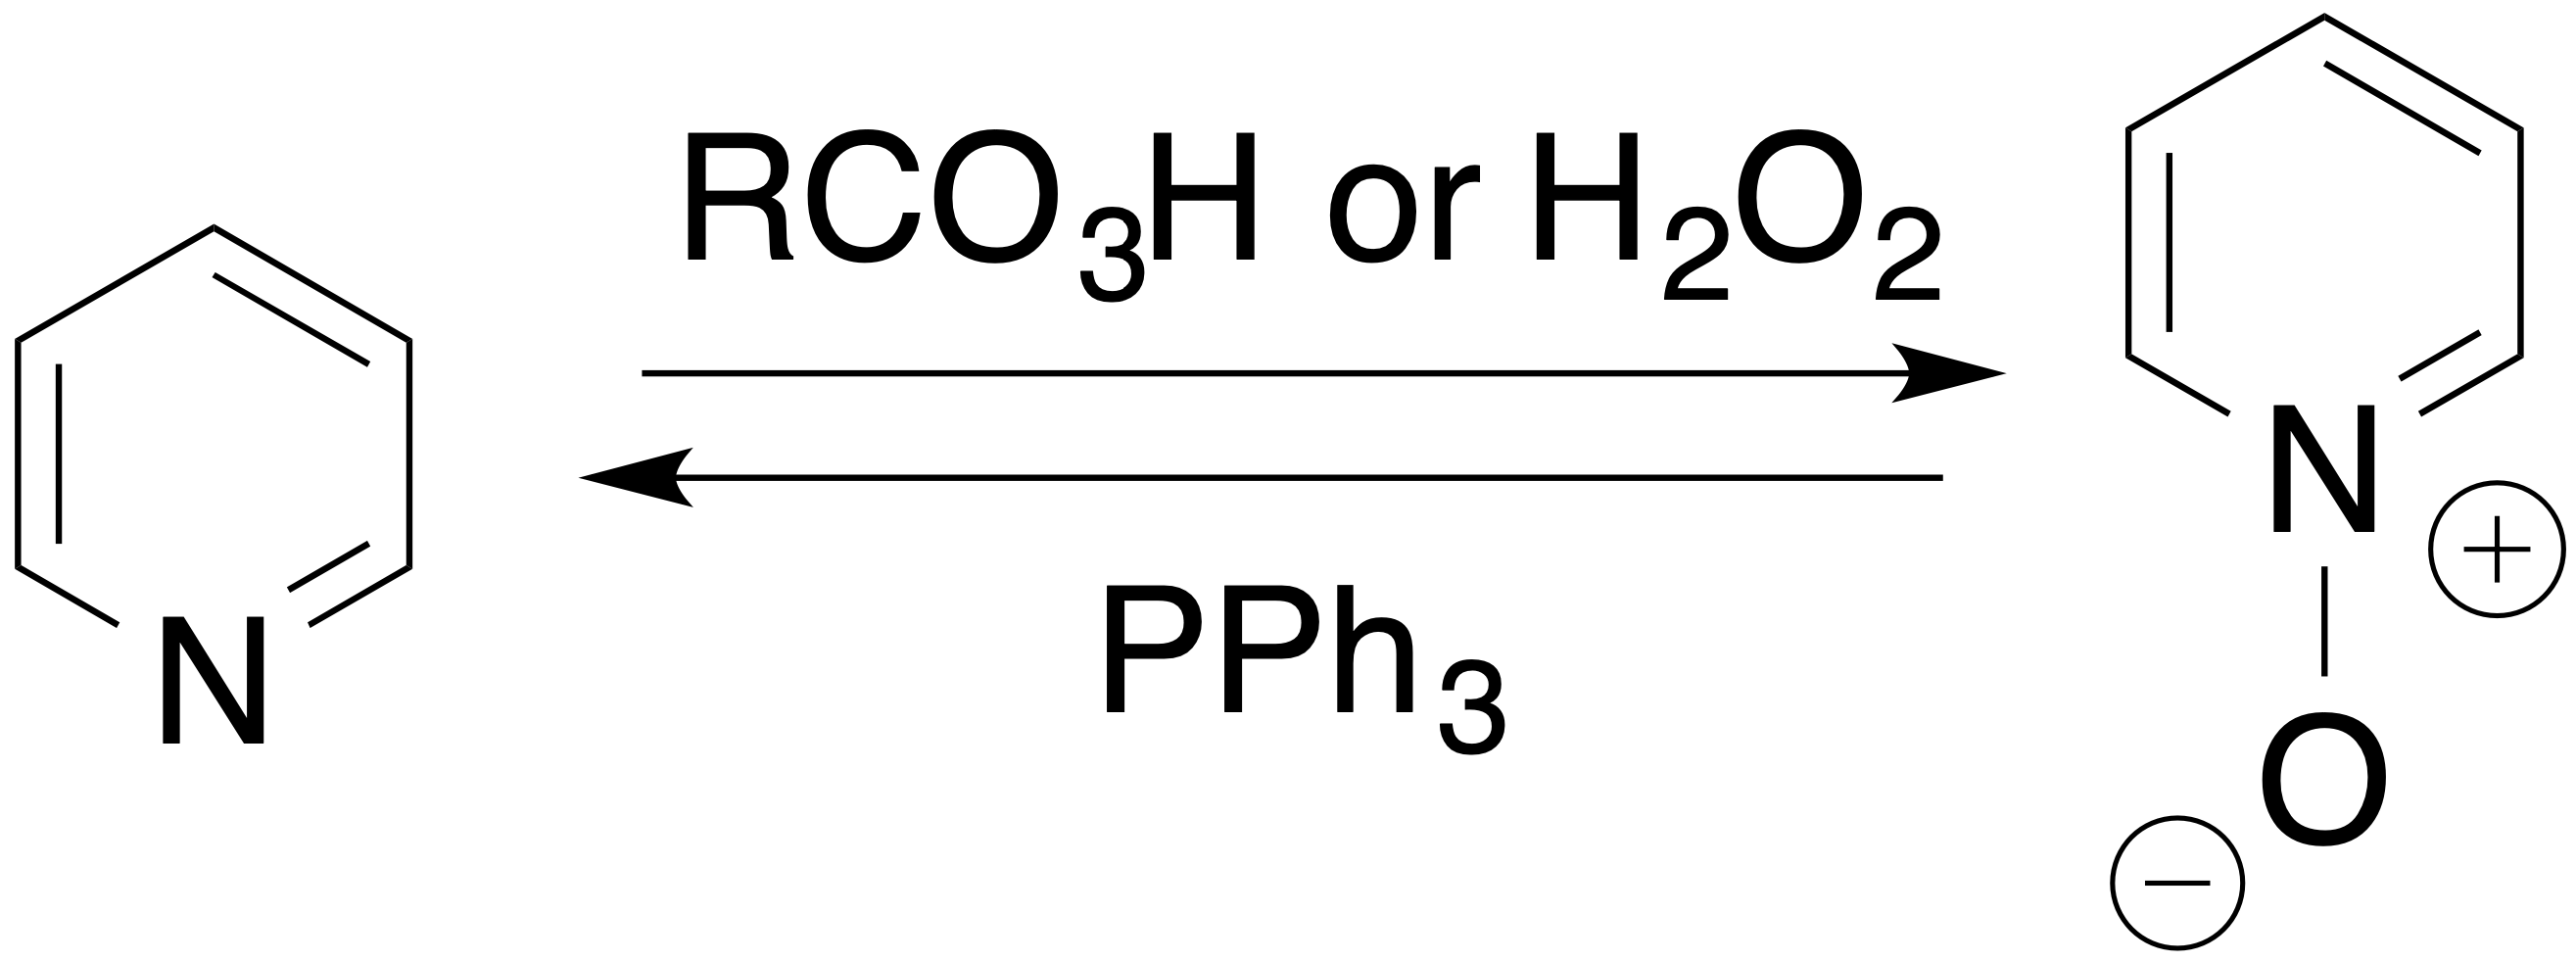
\includegraphics[width=0.3\linewidth]{PyNO.png}
        \caption{Synthesis of pyridine \emph{N}-oxides.}
        \label{fig:PyNO}
    \end{figure}
    \begin{itemize}
        \item Reversibly synthesize with peroxides, and \ce{PPh3}.
    \end{itemize}
    \item The counterintuitive result of pyridine oxidation is that the ring becomes \emph{more} electron-rich, because now the oxyanion's lone pairs donate in!
    \begin{itemize}
        \item Thus, for example, pyridine \emph{N}-oxide reacts under nitration conditions to yield 4-nitropyridine \emph{N}-oxide.
        \item As another example, \textbf{fuming sulfuric acid} and bromine lead to bromination at the 3-position.
        \begin{itemize}
            \item This is because the reaction is thought to proceed via oxygen coordination to \ce{HSO3+}.
        \end{itemize}
        \item \ce{POCl3} can also covert pyridine \emph{N}-oxide to 2-chloropyridine.
        \begin{itemize}
            \item BMS and Phil Baran have somewhat supplanted this reaction \parencite{bib:PyNOCl}.
        \end{itemize}
    \end{itemize}
    \item \textbf{Fuming sulfuric acid}: A mixture of \ce{H2SO4} and \ce{SO3}.
    \item We now move onto transition metal-catalyzed cross-coupling.
    \item TM-catalyzed cross-coupling has revolutionized the pharmaceutical industry, and somewhat distorted it.
    \begin{itemize}
        \item New drugs have a lot of biaryls because they're easy to make, probably not because they're optimal.
        \item Few reactions work with as much generality and substrate scope as cross-coupling.
    \end{itemize}
    \item Steve reviews the typical catalytic cycle for cross-coupling.
    \item Top reactions in the pharmaceutical industry.
    \begin{itemize}
        \item Amide-bond formation (huge!), and reductive amination.
    \end{itemize}
    \item List of cross-coupling reactions.
    \begin{itemize}
        \item Usually palladium- or nickel-catalyzed; some with copper.
        \item Kumada and Corriu developed a nickel-catalyzed cross-coupling that would have won the Nobel prize except that Kumada died.
        \item Negishi realized that a lot of magnesium reagents had functional group compatability issues.
        \begin{itemize}
            \item He went through zirconium before he got to zinc.
        \end{itemize}
        \item Stille probably had the best coupling, but he died in a plane crash. Functional group compatability and ease of separation of products is ideal with this, but it's not used as much any more due to toxicity concerns.
        \item Miyaura was an associate professor under Suzuki at Hokkaido who actually discovered this stuff.
        \begin{itemize}
            \item Most widely used because of ease and low toxicity.
        \end{itemize}
        \item Heck probably understood the chemistry the best; he was a remarkable individual in Steve's estimation.
        \begin{itemize}
            \item 7 single author back-to-back ($\times 7$) JACS publications.
            \begin{itemize}
                \item References: \textcite{bib:Heck1}, \textcite{bib:Heck2}, \textcite{bib:Heck3}, \textcite{bib:Heck4}, \textcite{bib:Heck5}, \textcite{bib:Heck6}, and \textcite{bib:Heck7}.
            \end{itemize}
            \item Timing is everything, and he published it too early.
            \item He was retired by the time he won the Nobel prize.
        \end{itemize}
        \item Ullmann was one of the first.
        \item Carbonylation: Aryl palladium with CO forms the acyl palladium that reacts just like an acid halide.
    \end{itemize}
    \item Ligands for CC.
    \begin{itemize}
        \item \ce{Pd(PPh3)4} is classic.
        \item Large bulky things turn out to be better.
        \item Having a bottom second ring (as in Buchwald ligands) also turns out to be useful.
        \item The principal: \ce{L4Pd} is unreactive; \ce{L2Pd} is quite good but hard to get to; \ce{L1Pd} is ideal. What the different ligands do is change the stability of the coordination environments. Buchwald ligands allow you to get down to \ce{L1Pd} species.
        \item Cone angle and percent buried volume are what is modulated by diarylbialkylphosphines.
        \item Trialkylphosphines and \emph{N}-heterocyclic carbenes can also be useful.
        \item References.
        \begin{itemize}
            \item \textcite{bib:BuchwaldRep} --- Steve's original report of SPhos and XPhos for Suzuki-Miyaura coupling.
            \item \textcite{bib:BuchwaldRev} --- Review of Steve's dialkylphosphinobiaryl ligands.
        \end{itemize}
    \end{itemize}
    \item Suzuki-Miyaura couplings.
    \begin{itemize}
        \item Hundreds of thousands of examples in the literature.
        \item Pd/C leaches a bit and can do the chemistry.
        \item You can also use ligands for more complicated stuff.
    \end{itemize}
\end{itemize}




\end{document}